% 建议使用 XeLaTeX 或 LuaLaTeX 编译(中文与公式支持更佳)
\documentclass[UTF8,zihao=-4]{ctexart}

% 版式与常用宏包
\usepackage[a4paper,margin=2.5cm]{geometry}
\usepackage{amsmath, amssymb, amsthm}
\usepackage{bm}
\usepackage{hyperref}
\usepackage{graphicx}
\usepackage{caption}
\usepackage{float} % 强制图表位置 [H]
\usepackage{placeins} % 控制浮动体不跨越屏障
\usepackage{listings}
\usepackage{xcolor}
\graphicspath{{figures/}}

% 代码样式
\lstdefinestyle{code}{
  basicstyle=\ttfamily\small,
  numbers=left,
  numberstyle=\tiny,
  numbersep=8pt,
  keywordstyle=\color{blue},
  commentstyle=\color{teal!70!black},
  stringstyle=\color{orange!70!black},
  showstringspaces=false,
  breaklines=true,
  frame=single,
  framerule=0.3pt,
  rulecolor=\color{black!15}
}
\lstset{style=code}

\title{回归的正则化方法:岭回归、Lasso 与 Elastic Net}
\author{}
\date{\today}

\begin{document}
\maketitle

\section{引言}
正则化用于控制模型复杂度,以缓解过拟合并提升泛化。在线性回归中,常见方法包括岭回归(\(\ell_2\))、Lasso(\(\ell_1\))与 Elastic Net(两者的组合)。它们通过将系数向零收缩来降低方差;其中 Lasso 还能产生稀疏性,从而实现嵌入式特征选择。

\section{原理与公式}
\subsection{模型}
给定特征 \(\mathbf{x}\in\mathbb{R}^d\),预测 \(\hat{y}=\mathbf{w}^\top\mathbf{x}+b\)。通常不对截距 \(b\) 加正则。

\subsection{岭回归(\(\ell_2\))}
\begin{equation}
\min_{\mathbf{w},b}\; \frac{1}{2n}\lVert \mathbf{X}\mathbf{w}+b\mathbf{1}-\mathbf{y} \rVert_2^2 + \frac{\lambda}{2}\lVert \mathbf{w} \rVert_2^2.
\end{equation}
在不惩罚截距时,可写闭式解 \(\mathbf{w}^*=(\mathbf{X}^\top\mathbf{X}+\lambda\mathbf{I})^{-1}\mathbf{X}^\top(\mathbf{y}-\bar{y}\mathbf{1})\)。岭回归连续收缩系数、缓解多重共线性,但不产生严格的零系数。

\subsection{Lasso(\(\ell_1\))}
\begin{equation}
\min_{\mathbf{w},b}\; \frac{1}{2n}\lVert \mathbf{X}\mathbf{w}+b\mathbf{1}-\mathbf{y} \rVert_2^2 + \lambda \lVert \mathbf{w} \rVert_1.
\end{equation}
鼓励稀疏(部分 \(w_j=0\))。由次梯度/KKT 条件可知:当残差与特征的相关性落入 \([-\lambda,\lambda]\) 带内时,对应系数会被压为零。

\subsection{Elastic Net}
结合 \(\ell_1\) 与 \(\ell_2\):
\begin{equation}
\min_{\mathbf{w},b}\; \frac{1}{2n}\lVert \mathbf{X}\mathbf{w}+b\mathbf{1}-\mathbf{y} \rVert_2^2 + \lambda\Big(\alpha\lVert \mathbf{w} \rVert_1 + \frac{1-\alpha}{2}\lVert \mathbf{w} \rVert_2^2\Big),\; \alpha\in[0,1].
\end{equation}
在强相关特征场景下更稳健:\(\ell_2\) 部分提升稳定性,\(\ell_1\) 保持稀疏。

\subsection{标准化与截距}
建议对特征逐列标准化、对 \(\mathbf{y}\) 去中心化;截距 \(b\) 不加正则并在居中数据上单独估计。

\subsection{优化}
岭回归可用闭式解或 QR/SVD;Lasso 与 Elastic Net 常用坐标下降与软阈值(配合热启动与递减 \(\lambda\) 路径)。

\section{应用场景与要点}
\begin{itemize}
  \item \textbf{多重共线性}:优先考虑岭回归或 Elastic Net 提升稳定性;
  \item \textbf{特征选择与可解释性}:Lasso/Elastic Net 能产生稀疏解;
  \item \textbf{模型选择}:通过交叉验证选择 \(\lambda\)/\(\alpha\),结合系数路径与验证曲线判断;
  \item \textbf{预处理}:标准化、异常值处理、根据业务对特征进行分组与筛选。
\end{itemize}

\section{Python 实战:Ridge 与 Lasso 系数路径}
本示例生成合成数据,并分别绘制 Lasso 与岭回归的系数路径,保存为 \texttt{figures/lasso\_path.png} 与 \texttt{figures/ridge\_path.png}。

\begin{lstlisting}[language=Python,caption={gen_regularization_figures.py}]
import os
import numpy as np
import matplotlib.pyplot as plt
from sklearn.linear_model import lasso_path, Ridge

np.random.seed(7)

n, d = 120, 12
X_raw = np.random.randn(n, d)
X_raw[:, 1] = 0.7*X_raw[:, 0] + 0.3*np.random.randn(n)

true_w = np.zeros(d)
true_w[[0, 3, 7]] = [2.0, -3.0, 1.5]
y = X_raw @ true_w + 0.8*np.random.randn(n)

# 标准化特征、去中心化 y
X = (X_raw - X_raw.mean(axis=0)) / X_raw.std(axis=0)
y = y - y.mean()

# Lasso 路径(alpha 递减)
alphas_lasso, coefs_lasso, _ = lasso_path(X, y, alphas=None)

fig, ax = plt.subplots(figsize=(7, 4.5))
for j in range(d):
    ax.plot(alphas_lasso, coefs_lasso[j, :], lw=1.6, label=f"w{j}")
ax.set_xscale('log'); ax.invert_xaxis()
ax.set_xlabel('alpha (log)'); ax.set_ylabel('coefficient')
ax.set_title('Lasso coefficient paths')
handles, labels = ax.get_legend_handles_labels()
ax.legend(handles[:6], labels[:6], loc='best', fontsize=8)

fig_dir = os.path.join(
    "0_Machine Learning", "0_Supervised Learning", "1_Regularization Methods in Regression", "figures")
os.makedirs(fig_dir, exist_ok=True)
plt.tight_layout(); plt.savefig(os.path.join(fig_dir, 'lasso_path.png'), dpi=160)

# 岭回归路径:不同 alpha 的系数
alphas_ridge = np.logspace(-3, 2, 40)
coefs_ridge = []
for a in alphas_ridge:
    model = Ridge(alpha=a, fit_intercept=False)
    model.fit(X, y)
    coefs_ridge.append(model.coef_)
coefs_ridge = np.array(coefs_ridge)

fig, ax = plt.subplots(figsize=(7, 4.5))
for j in range(d):
    ax.plot(alphas_ridge, coefs_ridge[:, j], lw=1.6, label=f"w{j}")
ax.set_xscale('log'); ax.invert_xaxis()
ax.set_xlabel('alpha (log)'); ax.set_ylabel('coefficient')
ax.set_title('Ridge coefficient paths')
handles, labels = ax.get_legend_handles_labels()
ax.legend(handles[:6], labels[:6], loc='best', fontsize=8)

plt.tight_layout(); plt.savefig(os.path.join(fig_dir, 'ridge_path.png'), dpi=160)
print('saved to', os.path.join(fig_dir, 'lasso_path.png'), 'and ridge_path.png')
\end{lstlisting}

\section{运行效果}
图~\ref{fig:lasso_path} 与图~\ref{fig:ridge_path} 展示了系数随正则强度变化的路径:Lasso 产生稀疏;岭回归连续收缩但不为零。

\begin{figure}[H]
  \centering
  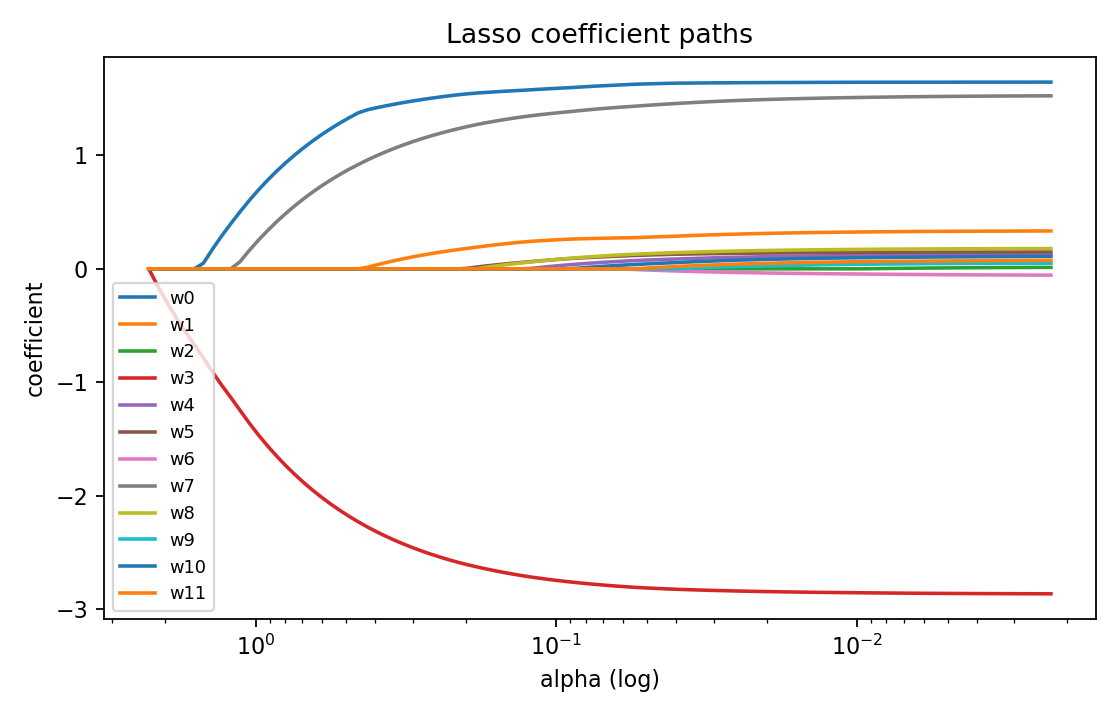
\includegraphics[width=0.85\linewidth]{lasso_path.png}
  \caption{Lasso 系数路径(合成数据)}
  \label{fig:lasso_path}
\end{figure}

\begin{figure}[H]
  \centering
  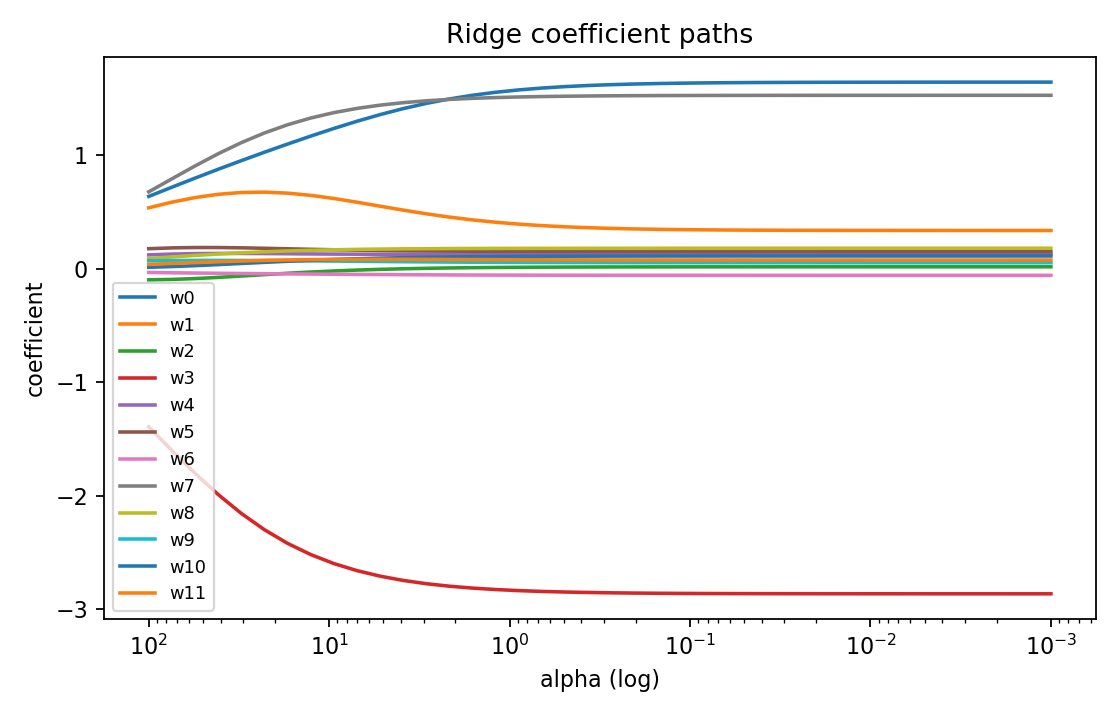
\includegraphics[width=0.85\linewidth]{ridge_path.png}
  \caption{岭回归系数路径(合成数据)}
  \label{fig:ridge_path}
\end{figure}

\FloatBarrier % 阻止上面的图漂移到后续章节

\section{小结}
正则化通过收缩系数来控制方差并提升泛化:多重共线性偏好岭回归,追求稀疏与可解释性使用 Lasso,强相关特征时考虑 Elastic Net。务必进行标准化,并通过交叉验证选择超参数。

\end{document}

